% !TeX program = lualatex
% Compile from this directory with:
%   latexmk -lualatex report.tex
% [DOC:DOCMETA-01] LaTeX 2026 document metadata and list-key activation.
\DocumentMetadata{lang=ja-JP,tagging=off}
\documentclass{ltjsarticle}

% guide_modules_start
% [DOC:MODULE-CORE-01] Core template configuration.
% !TeX root = ../report.tex

% Core language, layout, and document packages.
\usepackage[deluxe]{luatexja-preset}
\usepackage{graphicx}
\usepackage{geometry,tabularx}
\usepackage{fancyhdr}
\usepackage[labelformat=simple]{subcaption}
\usepackage{multirow}
\usepackage{booktabs}
\usepackage{float}
\usepackage{mathtools,amssymb}
\usepackage{xcolor}
\usepackage[sorting=none,bibstyle=ieee,citestyle=numeric-comp]{biblatex-jareport}
\usepackage[hidelinks]{hyperref}
\usepackage[sort&compress,nameinlink,noabbrev]{cleveref}

% Optional modules. Uncomment only the features used by a report.
% \input{config/diagrams}
% \input{config/listings}
% \input{config/plots}

% Page layout.
\geometry{top=25mm,bottom=30mm,left=25mm,right=25mm,footskip=12mm}
\setlength{\headheight}{30pt}
\renewcommand\thesubfigure{(\alph{subfigure})}

% Show equation numbers only when referenced. These wrappers preserve the
% normal cleveref interface, including starred and range commands.
\mathtoolsset{showonlyrefs=true}
\makeatletter
\NewCommandCopy{\labreport@cref}{\cref}
\NewCommandCopy{\labreport@Cref}{\Cref}
\NewCommandCopy{\labreport@crefrange}{\crefrange}
\NewCommandCopy{\labreport@Crefrange}{\Crefrange}

\RenewDocumentCommand{\cref}{s m}{%
  \noeqref{#2}%
  \IfBooleanTF{#1}
    {\labreport@cref*{#2}}
    {\labreport@cref{#2}}}

\RenewDocumentCommand{\Cref}{s m}{%
  \noeqref{#2}%
  \IfBooleanTF{#1}
    {\labreport@Cref*{#2}}
    {\labreport@Cref{#2}}}

\RenewDocumentCommand{\crefrange}{s m m}{%
  \noeqref{#2,#3}%
  \IfBooleanTF{#1}
    {\labreport@crefrange*{#2}{#3}}
    {\labreport@crefrange{#2}{#3}}}

\RenewDocumentCommand{\Crefrange}{s m m}{%
  \noeqref{#2,#3}%
  \IfBooleanTF{#1}
    {\labreport@Crefrange*{#2}{#3}}
    {\labreport@Crefrange{#2}{#3}}}
\makeatother

% Do not print an empty bibliography in the clean template.
\newif\iflabreporthasreferences
\AtDataInput{\global\labreporthasreferencestrue}

% Japanese cross-reference names and punctuation.
\crefname{figure}{図}{図}
\crefname{table}{表}{表}
\crefname{equation}{式}{式}
\crefname{section}{節}{節}
\crefname{subsection}{節}{節}
\crefname{subfigure}{図}{図}
\crefname{listing}{リスト}{リスト}
\crefname{lstlisting}{リスト}{リスト}
\Crefname{listing}{リスト}{リスト}
\Crefname{lstlisting}{リスト}{リスト}

\crefformat{figure}{図#2#1#3}
\crefformat{table}{表#2#1#3}
\crefformat{equation}{式#2(#1)#3}
\crefformat{listing}{リスト#2#1#3}
\crefformat{lstlisting}{リスト#2#1#3}

\crefrangeformat{figure}{図#3#1#4〜#5#2#6}
\crefrangeformat{subfigure}{図#3#1#4〜#5#2#6}
\AtBeginDocument{%
  \renewcommand{\crefrangeconjunction}{〜}%
  \renewcommand{\crefpairconjunction}{および}%
  \renewcommand{\crefmiddleconjunction}{、}%
  \renewcommand{\creflastconjunction}{および}%
  \renewcommand{\crefpairgroupconjunction}{および}%
  \renewcommand{\crefmiddlegroupconjunction}{、}%
  \renewcommand{\creflastgroupconjunction}{および}%
}

% [DOC:MODULE-DIAGRAMS-01] Optional diagram module.
% !TeX root = ../report.tex
% Optional TikZ, logic-circuit, and framed-content support.

\usepackage{tikz}
\usetikzlibrary{positioning,calc,arrows.meta,circuits.logic.US}
\usepackage{circuitikz}
\usepackage[framemethod=tikz]{mdframed}

% TeX Live 2026 replaces \item at begin-document time. mdframed still starts
% an internal legacy trivlist, so keep its matching legacy \item locally.
\makeatletter
\let\labreport@legacyitem\item
\pretocmd{\mdf@trivlist}{\let\item\labreport@legacyitem}{}{}
\makeatother

% [DOC:MODULE-LISTINGS-01] Optional source-code module.
% !TeX root = ../report.tex
% Optional source-code listing support.

\usepackage{listings}

\lstset{
  basicstyle=\ttfamily\fontsize{8}{10}\selectfont,
  frame=single,
  breaklines=true,
  columns=fullflexible,
  numbers=left,
  numberstyle=\tiny,
  keywordstyle=\color{blue},
  commentstyle=\color{gray},
  stringstyle=\color{red},
  captionpos=b,
  showstringspaces=false
}
\renewcommand{\lstlistingname}{リスト}
\renewcommand{\lstlistlistingname}{リスト一覧}

% [DOC:MODULE-PLOTS-01] Optional PGFPlots module.
% !TeX root = ../report.tex
% Optional PGFPlots styles for laboratory-report graphs.

\usepackage{pgfplots}

\pgfplotsset{compat=1.18}
\definecolor{plotLine}{HTML}{4F4F4F}
\pgfplotsset{
  report axis base/.style={
    width=0.78\linewidth,
    height=0.50\linewidth,
    scale only axis,
    axis lines=box,
    axis background/.style={fill=white},
    axis line style={black, line width=0.8pt},
    grid=major,
    major grid style={draw=black!25, line width=0.25pt},
    minor tick num=1,
    tick pos=left,
    tick align=inside,
    tick style={black, line width=0.7pt},
    major tick length=3pt,
    minor tick length=1.8pt,
    xticklabel style={
      font=\small,
      /pgf/number format/fixed,
      /pgf/number format/precision=1
    },
    yticklabel style={
      font=\small,
      /pgf/number format/fixed,
      /pgf/number format/precision=1
    },
    label style={font=\normalsize},
    xlabel style={yshift=-2mm},
    ylabel style={yshift=1mm}
  },
  report legend/.style={
    legend pos=north west,
    legend cell align=left,
    legend style={
      font=\footnotesize,
      draw=black,
      fill=white,
      line width=0.4pt,
      inner xsep=3pt,
      inner ysep=2pt,
      row sep=1pt
    },
    legend image code/.code={
      \draw[mark repeat=2, mark phase=2, ##1]
        plot coordinates {(0cm,0cm) (0.25cm,0cm) (0.5cm,0cm)};
    }
  },
  report axis/.style={
    report axis base,
    report legend
  },
  report plot/.style={
    plotLine,
    line width=1.2pt,
    mark size=2.1pt,
    mark options={solid, fill=plotLine, draw=plotLine}
  },
  report dual right axis/.style={
    report axis base,
    axis y line*=right,
    axis x line=none,
    axis background/.style={fill=none},
    grid=none,
    tick pos=right,
    ytick pos=right,
    yticklabel pos=right,
    ylabel style={
      at={(axis description cs:1.14,0.5)},
      % PGFPlots already rotates y labels by 90 degrees; flip the right label.
      rotate=180,
      anchor=north
    }
  }
}

% [DOC:MODULE-COMMANDS-01] Public report metadata commands.
% !TeX root = ../report.tex

\makeatletter

\newcommand{\course}[1]{\def\@course{#1}}
\newcommand{\group}[1]{\def\@group{#1}}
\newcommand{\theme}[1]{\def\@theme{#1}}
\newcommand{\studentid}[1]{\def\@studentid{#1}}
\newcommand{\experimentpartner}[1]{\def\@experimentpartner{#1}}
\newcommand{\staff}[1]{\def\@staff{#1}}
\newcommand{\experimentdate}[1]{\def\@experimentdate{#1}}
\newcommand{\place}[1]{\def\@place{#1}}
\newcommand{\experimenttime}[1]{\def\@experimenttime{#1}}
\newcommand{\reportfirstdue}[1]{\def\@reportfirstdue{#1}}

\providecommand{\@course}{}
\providecommand{\@group}{}
\providecommand{\@theme}{}
\providecommand{\@studentid}{}
\providecommand{\@experimentpartner}{}
\providecommand{\@staff}{}
\providecommand{\@experimentdate}{}
\providecommand{\@place}{}
\providecommand{\@experimenttime}{}
\providecommand{\@reportfirstdue}{}

\renewcommand{\maketitle}{%
  \begin{center}
    {\Large \bfseries レポートの基本情報\par}
    \vspace{1em}
    \begin{tabularx}{0.95\linewidth}{@{}>{\raggedright\arraybackslash}p{0.25\linewidth}
                                    >{\centering\arraybackslash}m{1em}
                                    >{\raggedright\arraybackslash}X@{}}
      \hline
      実験テーマ名 & ： & \@title \\
      レポート執筆者 & ： & \@author \\
      共同実験者 & ： & \@experimentpartner \\
      担当教員やTA名 & ： & \@staff \\
      実験実施日 & ： & \@experimentdate \\
      実施場所 & ： & \@place \\
      時間 & ： & \@experimenttime \\
      初回提出日 & ： & \@reportfirstdue \\
      \hline
    \end{tabularx}
  \end{center}
}

\pagestyle{fancy}
\fancyhf{}
\fancyhead[C]{%
  \small
  \begingroup
  \renewcommand{\arraystretch}{0.95}%
  \begin{tabularx}{\textwidth}{@{}
      >{\raggedright\arraybackslash}m{0.26\textwidth}
      >{\centering\arraybackslash}m{0.10\textwidth}
      >{\centering\arraybackslash}m{0.19\textwidth}
      >{\centering\arraybackslash}m{0.08\textwidth}
      >{\raggedleft\arraybackslash}X@{}}
    \@course & テーマ\ \@theme & 学籍番号：\@studentid & \@group 班 & 作成者：\@author
  \end{tabularx}%
  \endgroup
}
\fancyfoot[C]{\thepage}
\makeatother

% guide_modules_end

% [DOC:GUIDE-TOGGLE-01]
% SAMPLE-ONLY: Set this false to compile only the black experiment report.
\newif\ifshowsampleguide
\showsampleguidetrue
% !TeX root = ../report.tex
% SAMPLE-ONLY: This file builds the explanatory layer in the annotated example.
% These commands and styles are not part of the LabReportTex template interface.

% [DOC:COLOR-ANNOTATION-01] Colored notes kept separate from the black report body.
\NewDocumentCommand{\SampleGuideNote}{O{blue!65!black} m +m}{%
  \ifshowsampleguide
    \par\smallskip
    {\small\color{#1}\noindent
      \textbf{#2}\quad #3\par}%
  \fi
}

\lstdefinestyle{sample guide source}{
  language={[LaTeX]TeX},
  basicstyle=\ttfamily\fontsize{7.2}{9}\selectfont,
  frame=single,
  framerule=0.5pt,
  rulecolor=\color{black!35},
  backgroundcolor=\color{black!3},
  breaklines=true,
  columns=fullflexible,
  numbers=none,
  keywordstyle=\color{blue!65!black},
  commentstyle=\color{green!35!black},
  stringstyle=\color{red!65!black},
  showstringspaces=false,
  xleftmargin=0.5em,
  xrightmargin=0.5em,
  aboveskip=0.35em,
  belowskip=0.6em
}

% [DOC:GUIDE-SOURCE-01] Exact source ranges printed beside their PDF results.
\NewDocumentCommand{\SampleGuideSource}{O{} m m m m}{%
  \ifshowsampleguide
    \par\smallskip
    {\small\color{black!65}\noindent
      \textbf{#2}\quad
      \texttt{\detokenize{#3}}\par}%
    \lstinputlisting[
      style=sample guide source,
      linerange={#4-#5},
      includerangemarker=false,
      #1
    ]{#3}%
  \fi
}

% !TeX root = ../report.tex
% guide_metadata_start
% [DOC:META-TITLE-01]
\title{RC低域通過フィルタの周波数特性}
% [DOC:META-AUTHOR-01]
\author{サンプル作成者}

% [DOC:META-COURSE-01]
\course{電気電子工学基礎実験}
% [DOC:META-GROUP-01]
\group{A}
% [DOC:META-THEME-01]
\theme{04}
% [DOC:META-STUDENT-01]
\studentid{000000000}
% [DOC:META-PARTNER-01]
\experimentpartner{サンプル共同実験者}
% [DOC:META-STAFF-01]
\staff{サンプル担当者}
% [DOC:META-DATE-01]
\experimentdate{20XX年6月12日}
% [DOC:META-PLACE-01]
\place{電気電子実験室}
% [DOC:META-TIME-01]
\experimenttime{13:00--16:10}
% [DOC:META-DUE-01]
\reportfirstdue{20XX年6月19日}
% guide_metadata_end


% [DOC:BIB-RESOURCE-01] Bibliography database used by this example.
\addbibresource{bibliography/references.bib}
% [DOC:GRAPHICSPATH-01] Search external image assets under figures/.
\graphicspath{{figures/}}

\begin{document}

% !TeX root = ../report.tex
% SAMPLE-ONLY: \SampleGuideNote adds PDF guidance and is not a template command.
% [DOC:NOTICE-01] One-sentence notice before the title information table.
% [DOC:BIB-REPOSITORY-01] First citation points to the public project repository.
\SampleGuideNote[purple!70!black]{サンプルについて}{%
以下は LabReportTex を用いて作成した架空の実験例です\cite{labreporttex}。}
\smallskip


% [DOC:TITLEBLOCK-01] Template-specific title information table.
\maketitle

% [DOC:META-TITLE-AUTHOR-01] Visible title/author and PDF metadata result.
\SampleGuideNote[purple!70!black]{この PDF の読み方}{%
  黒い文章だけを読むと、一つの実験レポートになります。色付きの文章では使い方を短く説明し、
  灰色の枠には実際に使ったソースを示します。詳しい仕組みを確認したい場合は、
  プロジェクトの説明文書とサンプルソースをご覧ください。}

\SampleGuideNote[purple!70!black]{［META-TITLE-AUTHOR-01］}{%
  レポート名と作成者は \texttt{config/metadata.tex} で変更します。
  ここに書いた内容は基本情報表に表示され、PDF のタイトルと作成者にも保存されます。}

\SampleGuideSource
  {レポート情報を入力している部分}
  {config/metadata.tex}
  {guide_metadata_start}
  {guide_metadata_end}

\SampleGuideNote[purple!70!black]{灰色のソース欄について}{%
  灰色の枠は、このサンプル PDF だけで使う説明機能です。空のテンプレートには含まれていません。
  枠内のコードは、上の基本情報表を実際に作るときに読み込まれたものです。}

% [DOC:META-HEADER-01] Metadata fields displayed in the running header.
% [DOC:META-TABLE-01] Metadata fields displayed by maketitle.
\SampleGuideNote[purple!70!black]{基本情報の表示場所}{%
  科目名、テーマ番号、学籍番号、班は各ページの上部にも表示されます。
  共同実験者、担当者、実施日時、場所、提出日は、最初の基本情報表で確認できます。}

% [DOC:LAYOUT-HEADER-01] fancyhdr page style.
% [DOC:LAYOUT-PAGE-01] geometry page layout.
\SampleGuideNote[purple!70!black]{ページ上部と余白}{%
  ページ上部の情報と下部中央のページ番号は、テンプレートが自動で配置します。
  余白も全ページで同じ設定になるため、通常は各章で個別に調整する必要はありません。}

% [DOC:CORE-JAPANESE-01] Japanese, Latin, numeric, and math composition.
\SampleGuideNote[purple!70!black]{日本語と文書設定}{%
  このテンプレートは LuaLaTeX で日本語を組版します。
  文書の最初にある \texttt{\string\DocumentMetadata} は、PDF の言語を日本語に設定し、
  この例で使う新しいリスト設定も有効にします。}

% [DOC:MODULES-01] Optional module entry points.
\SampleGuideSource
  {テンプレート設定を読み込んでいる部分}
  {report.tex}
  {guide_modules_start}
  {guide_modules_end}

\SampleGuideNote[purple!70!black]{設定ファイルの読み込み}{%
  基本設定とレポート情報用の命令は常に読み込みます。
  このサンプルでは、回路図、コード、グラフも使うため、三つの追加設定を読み込んでいます。
  \texttt{config/sample-guide.tex} だけは説明表示専用で、テンプレート本体の機能ではありません。}

% SAMPLE-ONLY: \SampleGuideNote and \SampleGuideSource are not template commands.
\section{目的}
\label{sec:purpose}

\subsection{実験の背景}
\label{subsec:background}

温度センサの出力を記録する予備観察では、ゆっくり変化する信号に加えて、
数 \unit{\kilo\hertz} 付近の細かな振動が重なって表示された。
この振動が記録値の読み取りを不安定にするため、測定信号から高い周波数成分を
減衰させる前処理回路が必要になった。

抵抗とコンデンサで構成される一次 RC 低域通過フィルタは、
少ない素子で構成でき、遮断周波数を素子値から直接予測できる。
そこで本実験では、RC 低域通過フィルタを実際に構成し、入力周波数を変化させたときの
出力振幅と位相差を測定することにした。

低い周波数では出力が入力にほぼ追従し、遮断周波数付近では利得が
\qty{-3}{\decibel}、位相差が \ang{-45} 付近になると予想した。
さらに高い周波数では、周波数が 10 倍になるごとに利得がおよそ
\qty{20}{\decibel} 低下し、位相差は \ang{-90} に近づくと考えた。

% [DOC:STRUCT-SECTION-01] Section and subsection hierarchy.
\SampleGuideNote[purple!70!black]{見出し構造の補足}{%
本文は \texttt{\string\section} と \texttt{\string\subsection} で段階的に分け、
  各見出しに \texttt{\string\label} を付けています。}

\subsection{到達目標}
\label{subsec:objectives}

本実験の到達目標を以下に示す。

% [DOC:LIST-ITEMIZE-01] Itemized experimental objectives.
% guide_itemize_start
\begin{itemize}[leftmargin=2.8em,nosep]
  \item RC 低域通過フィルタの振幅特性と位相特性を測定する。
  \item 測定した素子値から遮断周波数を予測する。
  \item 利得、位相差および曲線近似から遮断周波数を推定する。
  \item 理論値と測定値の差を整理し、主な誤差要因を検討する。
\end{itemize}
% guide_itemize_end

\SampleGuideSource
  {目標を箇条書きにするコード}
  {sections/01-purpose.tex}
  {guide_itemize_start}
  {guide_itemize_end}

\SampleGuideNote[teal!70!black]{［LIST-ITEMIZE-01］}{%
順番を付けずに項目を並べるときは、\texttt{itemize} を使います。
各項目は \texttt{\string\item} から書き始めます。}

% [DOC:LIST-KEY-LEFTMARGIN-01] New list key for the left margin.
\SampleGuideNote[teal!70!black]{左余白の補足}{%
\texttt{leftmargin=2.8em} で、リスト全体の左側の空きを調整しています。}

% [DOC:LIST-KEY-NOSEP-01] New list key for compact spacing.
\SampleGuideNote[teal!70!black]{項目間隔の補足}{%
\texttt{nosep} を付けると、項目どうしの間隔を小さくできます。}

\subsection{確認する量}
\label{subsec:observables}

実験中に直接読み取る量と、測定後に計算する量を区別した。
直接読み取る量は入力振幅、出力振幅、二つの波形の時間差である。
これらを用いて、次の量を比較する。

% [DOC:LIST-ITEMIZE-02] A second itemize example with more spacing.
\begin{itemize}[leftmargin=3.2em,itemsep=0.35em]
  \item 振幅比 $V_{\mathrm{out}}/V_{\mathrm{in}}$
  \item デシベル表示の利得 $G$
  \item 入出力間の位相差 $\phi$
  \item 利得残差 $G_{\mathrm{measured}}-G_{\mathrm{theory}}$
  \item 三回の繰り返し測定から求める標準偏差
\end{itemize}

\SampleGuideNote[teal!70!black]{同じリストを使い分ける例}{%
同じ \texttt{itemize} でも、\texttt{itemsep} を指定すると各項目の間隔を広げられます。}

以上の量を用いて、通過域、遷移域、減衰域の特徴を順に確認する。
理論式は\cref{sec:theory}、装置と手順は\cref{sec:method}、測定値は
\cref{sec:results}、測定値の解釈は\cref{sec:discussion}に示す。

% [DOC:REF-SECTION-01] Section references with cleveref.
\SampleGuideNote[blue!65!black]{［REF-SECTION-01］}{%
節のラベルを \texttt{\string\cref} に渡すと、「節」を含む参照を自動で出力できます。}

\SampleGuideNote[blue!65!black]{複数の節を参照する場合}{%
複数の節を個別に参照しても、リンク先は各 \texttt{\string\label} に対応します。}

% SAMPLE-ONLY: \SampleGuideNote and \SampleGuideSource are not template commands.
\section{原理}
\label{sec:theory}

\subsection{複素インピーダンス}
\label{subsec:impedance}

抵抗とコンデンサから構成される一次 RC 低域通過フィルタを考える。
入力電圧を $V_{\mathrm{in}}$、コンデンサ両端の出力電圧を
$V_{\mathrm{out}}$ とする。複素数を用いた回路計算の基本的な整理は
複数の資料を参照した\cite{jp-book,jp-article,jp-inbook}。

角周波数を $\omega=2\pi f$、虚数単位を $j$ とすると、
コンデンサのインピーダンスは\cref{eq:capacitor}で表される。

% [DOC:MATH-EQUATION-01] A single numbered equation.
% guide_equation_start
\begin{equation}
  Z_C=\frac{1}{j\omega C}
  \label{eq:capacitor}
\end{equation}
% guide_equation_end

\SampleGuideSource
  {一つの数式を書くコード}
  {sections/02-theory.tex}
  {guide_equation_start}
  {guide_equation_end}

\SampleGuideNote[blue!65!black]{［MATH-EQUATION-01］}{%
一つの数式を独立して表示するときは \texttt{equation} を使います。
後から本文で参照するため、式の中に \texttt{\string\label} も付けています。}

複素周波数 $s$ を用いる場合、$s\in\mathbb{C}$ とし、定常正弦波では
$s=j\omega$ と置く。本実験で扱う周波数は $f\in\mathbb{R}_{>0}$ である。

% [DOC:MATH-AMSSYMB-01] Blackboard bold symbols from amssymb.
\SampleGuideNote[blue!65!black]{［MATH-AMSSYMB-01］}{%
\texttt{amssymb} が提供する \texttt{\string\mathbb} を使い、複素数全体と正の実数全体を表しています。}

\subsection{伝達関数}
\label{subsec:transfer}

抵抗とコンデンサの直列回路に分圧則を適用する。
伝達関数を $H(j\omega)\coloneqq V_{\mathrm{out}}/V_{\mathrm{in}}$ と定義すると、
導出過程は\crefrange{eq:divider}{eq:transfer}となる。

% [DOC:MATH-ALIGN-01] Multi-line aligned derivation.
% guide_align_start
\begin{align}
  V_{\mathrm{out}}
    &=\frac{Z_C}{R+Z_C}V_{\mathrm{in}}
      \label{eq:divider}\\
  H(j\omega)
    &\coloneqq\frac{V_{\mathrm{out}}}{V_{\mathrm{in}}}
      \label{eq:definition}\\
    &=\frac{Z_C}{R+Z_C}
      \label{eq:substitution}\\
    &=\frac{1}{1+j\omega RC}.
      \label{eq:transfer}
\end{align}
% guide_align_end

\SampleGuideSource
  {複数行の式をそろえるコード}
  {sections/02-theory.tex}
  {guide_align_start}
  {guide_align_end}

\SampleGuideNote[blue!65!black]{［MATH-ALIGN-01］}{%
複数行の式で等号の位置をそろえるときは \texttt{align} を使います。
\texttt{\&} を置いた位置が縦にそろい、必要な行にはそれぞれラベルを付けられます。}

% [DOC:MATH-COLONEQQ-01] Definition symbol from mathtools.
\SampleGuideNote[blue!65!black]{数式の補足}{%
\texttt{\string\coloneqq} は「ここで定義する」ことを明示する \texttt{mathtools} の記号です。}

% [DOC:REF-RANGE-01] Lowercase range reference.
\SampleGuideNote[blue!65!black]{［REF-RANGE-01］}{%
連続する式をまとめて示す場合は \texttt{\string\crefrange} を使います。ここでは式の開始番号と終了番号が範囲表示になります。}

\subsection{振幅特性と位相特性}
\label{subsec:frequency-characteristics}

\Cref{eq:transfer}の絶対値と偏角を求めると、振幅比、利得、位相差は
\crefrange{eq:magnitude}{eq:phase}で表される。

% [DOC:MATH-FREQUENCY-01] Magnitude, gain, and phase equations.
\begin{align}
  \lvert H(j\omega)\rvert
    &=\frac{1}{\sqrt{1+(\omega RC)^2}}
      \label{eq:magnitude}\\
  G
    &=20\log_{10}\lvert H(j\omega)\rvert
      \label{eq:gain}\\
  \phi
    &=-\tan^{-1}(\omega RC).
      \label{eq:phase}
\end{align}

% [DOC:REF-CAPITAL-01] Capitalized reference form.
\SampleGuideNote[blue!65!black]{［REF-CAPITAL-01］}{%
文頭から参照を始める場合は \texttt{\string\Cref} を使用できます。}

% [DOC:REF-NAME-01] Automatic Japanese reference names.
\SampleGuideNote[blue!65!black]{参照の補足}{%
\texttt{cleveref} はラベルの種類を判定し、式には「式」、図には「図」、表には「表」を自動で付けます。}

低周波数側と高周波数側の概略を比較するため、利得の漸近形を
\cref{eq:asymptotic-gain}に示す。

% [DOC:MATH-DCASES-01] Mathtools dcases environment.
\begin{equation}
  G(f)\simeq
  \begin{dcases}
    0, & f\ll f_c,\\
    -20\log_{10}\!\left(\frac{f}{f_c}\right), & f\gg f_c.
  \end{dcases}
  \label{eq:asymptotic-gain}
\end{equation}

\SampleGuideNote[blue!65!black]{［MATH-DCASES-01］}{%
条件によって式を分ける例では、\texttt{mathtools} の \texttt{dcases} を使用しています。}

\subsection{遮断周波数と時定数}
\label{subsec:cutoff}

振幅比が $1/\sqrt{2}$ となる周波数を遮断周波数 $f_c$ とする。
遮断周波数と時定数 $\tau$ は、\crefrange{eq:cutoff}{eq:tau}で表される。

\begin{align}
  f_c&=\frac{1}{2\pi RC}
    \label{eq:cutoff}\\
  \tau&=RC.
    \label{eq:tau}
\end{align}

抵抗の公称値 $1.00\,\mathrm{k}\Omega$、コンデンサの公称値 $0.100\,\mu\mathrm{F}$ を代入すると、予測値は\cref{eq:cutoff-nominal}となる。

\begin{equation}
  f_{c,\mathrm{nominal}}=1.59\times10^3\,\mathrm{Hz}
  \label{eq:cutoff-nominal}
\end{equation}

次の式は計算途中で用いた時定数であり、本文から参照していない。

% [DOC:MATH-SHOWONLYREFS-01] Deliberately unreferenced equation.
\begin{equation}
  RC=1.00\times10^{-4}\,\mathrm{s}
  \label{eq:time-constant-unreferenced}
\end{equation}

\SampleGuideNote[blue!65!black]{［MATH-SHOWONLYREFS-01］}{%
\texttt{showonlyrefs} により、本文から参照されない時定数の式には番号が表示されません。}

% [DOC:REF-STAR-01] Unlinked single references.
\SampleGuideNote[blue!65!black]{リンクなし参照の例}{%
星付き形式ではリンクを付けずに、\cref*{eq:cutoff}、\Cref*{eq:cutoff}のような参照文字列だけを出力できます。}

% [DOC:REF-RANGE-STAR-01] Unlinked range references.
\SampleGuideNote[blue!65!black]{リンクなし範囲参照の例}{%
範囲にも星付き形式があり、\crefrange*{eq:cutoff}{eq:tau}、
  \Crefrange*{eq:cutoff}{eq:tau}のように使用できます。}

\subsection{波形から求める位相差}
\label{subsec:phase-measurement}

オシロスコープで観測した二つの波形について、入力波形より出力波形が
$\Delta t$ だけ遅れたとする。一周期を $T=1/f$ とすれば、位相差は
\cref{eq:phase-delay}から計算できる。

\begin{equation}
  \phi=-360\frac{\Delta t}{T}=-360f\Delta t
  \label{eq:phase-delay}
\end{equation}

例えば $f=1.60\,\mathrm{kHz}$、$\Delta t=80\,\mathrm{\mu s}$ の場合、
$\phi\simeq-46\,\mathrm{deg}$ となる。

\subsection{素子公差による予測範囲}
\label{subsec:tolerance-range}

抵抗とコンデンサがそれぞれ公称値から変化すると、遮断周波数も変化する。
ここでは抵抗を $0.98$--$1.02\,\mathrm{k}\Omega$、コンデンサを
$0.095$--$0.105\,\mu\mathrm{F}$ の範囲として、上下限を計算した。

\begin{align}
  f_{c,\min}
    &=\frac{1}{2\pi R_{\max}C_{\max}}
      =1.49\,\mathrm{kHz}
      \label{eq:cutoff-min}\\
  f_{c,\max}
    &=\frac{1}{2\pi R_{\min}C_{\min}}
      =1.71\,\mathrm{kHz}.
      \label{eq:cutoff-max}
\end{align}

\Crefrange{eq:cutoff-min}{eq:cutoff-max}は、素子値だけから予想した遮断周波数の範囲である。

% [DOC:REF-RANGE-CAPITAL-01] Capitalized range reference form.
\SampleGuideNote[blue!65!black]{［REF-RANGE-CAPITAL-01］}{%
文頭で範囲参照を使う場合は \texttt{\string\Crefrange} を使用します。}

\subsection{記号と周波数領域}
\label{subsec:symbols}

% [DOC:LIST-DESCRIPTION-01] Description list for symbols.
本報告で使用する主な記号を以下にまとめる。
\begin{description}[leftmargin=8em,labelwidth=6.5em,nosep]
  \item[$R$] 抵抗値
  \item[$C$] 静電容量
  \item[$f$] 入力信号の周波数
  \item[$\omega$] 角周波数
  \item[$G$] デシベル表示の利得
  \item[$\phi$] 入出力間の位相差
  \item[$f_c$] 遮断周波数
  \item[$\tau$] 時定数
\end{description}

\SampleGuideNote[teal!70!black]{［LIST-DESCRIPTION-01］}{%
用語や記号と説明を対応させる場合は \texttt{description} 環境が使いやすいです。}

% [DOC:LIST-DESCRIPTION-02] A second description list for frequency regions.
測定結果は次の三領域に分けて整理する。
\begin{description}[leftmargin=8em,labelwidth=6.5em,itemsep=0.3em]
  \item[通過域] 利得が $0\,\mathrm{dB}$ に近く、入力信号がほぼ保たれる領域
  \item[遷移域] 利得と位相差が大きく変化し、遮断周波数を含む領域
  \item[減衰域] 高周波成分が明確に減衰する領域
\end{description}

\SampleGuideNote[teal!70!black]{説明リストの補足}{%
ラベル幅と左余白を別々に指定すると、長さの異なる用語でも説明文の開始位置をそろえられます。}

% SAMPLE-ONLY: \SampleGuideNote and \SampleGuideSource are not template commands.
\section{実験方法}
\label{sec:method}

\subsection{使用機器}
\label{subsec:equipment}

% [DOC:LIST-BASIC-01] Basic LaTeX list with explicit lengths.
使用機器と素子を以下に示す。
\begin{list}{--}{%
  \setlength{\leftmargin}{2.8em}%
  \setlength{\itemsep}{0.15em}%
  \setlength{\parsep}{0pt}%
}
  \item 信号発生器：Sample Generator A
  \item オシロスコープ：Sample Scope B
  \item デジタルマルチメータ：Sample Meter C
  \item 10 倍受動プローブ：2 本
  \item 金属皮膜抵抗：公称値 \qty{1.00}{\kilo\ohm}
  \item フィルムコンデンサ：公称値 \qty{0.100}{\micro\farad}
  \item ブレッドボード、接続線、BNC 変換端子
\end{list}

\SampleGuideNote[teal!70!black]{［LIST-BASIC-01］}{%
LaTeX の基本 \texttt{list} 環境では、第 1 引数にラベル、第 2 引数に余白や項目間隔を記述できます。}

各機器の主な設定と用途を\cref{tab:equipment}に示す。機器の仕様は、
校正記録と公開資料を参照して整理した\cite{jp-report,jp-online,jp-misc}。

% [DOC:TABLE-TABULARX-01] Instrument table with an X column.
% guide_equipment_table_start
\begin{table}[htbp]
  \centering
  \caption{使用機器の設定と用途}
  \label{tab:equipment}
  \begin{tabularx}{\linewidth}{
      >{\raggedright\arraybackslash}p{0.20\linewidth}
      >{\raggedright\arraybackslash}p{0.22\linewidth}
      >{\raggedright\arraybackslash}X}
    \toprule
    機器 & 主な設定 & 本実験での用途 \\
    \midrule
    信号発生器
      & 正弦波、\qty{1.00}{\volt}、出力抵抗 \qty{50}{\ohm}
      & \qty{100}{\hertz} から \qty{10}{\kilo\hertz} まで周波数を変化させ、RC 回路へ一定振幅の信号を入力する。\\
    オシロスコープ
      & 2 チャンネル、AC 結合、時間差カーソル
      & 入力波形と出力波形を同時に表示し、振幅と二つの波形の時間差を読み取る。\\
    デジタルマルチメータ
      & 抵抗測定、容量測定
      & 回路を構成する前に抵抗値と静電容量を三回ずつ測定する。\\
    10 倍プローブ
      & 入力容量 \qty{12}{\pico\farad}、入力抵抗 \qty{10}{\mega\ohm}
      & 回路への負荷を小さくしながら、入力側と出力側の電圧を測定する。\\
    \bottomrule
  \end{tabularx}
\end{table}
% guide_equipment_table_end

\SampleGuideSource
  {幅に合わせて文章を折り返す表のコード}
  {sections/03-method.tex}
  {guide_equipment_table_start}
  {guide_equipment_table_end}

\SampleGuideNote[orange!80!black]{［TABLE-TABULARX-01］}{%
\texttt{tabularx} の \texttt{X} 列は、表の残った幅を使います。
文章が長い場合は、列の中で自動的に折り返されます。}

\SampleGuideNote[orange!80!black]{固定幅列の補足}{%
最初の二列には折り返し可能な \texttt{p} 列を使い、機器名と設定の列幅を固定しています。}

\subsection{素子値の予備測定}
\label{subsec:component-measurement}

抵抗とコンデンサを回路へ取り付ける前に、それぞれ三回測定した。
端子に触れないように部品を固定し、測定値が安定してから記録した。
結果を\cref{tab:components}に示す。

% [DOC:TABLE-PCOLUMN-01] Fixed-width wrapping columns.
\begin{table}[H]
  \centering
  \caption{素子値の予備測定結果}
  \label{tab:components}
  \setlength{\tabcolsep}{3pt}
  \begin{tabularx}{\linewidth}{
      >{\centering\arraybackslash}p{0.13\linewidth}
      >{\centering\arraybackslash}p{0.11\linewidth}
      >{\centering\arraybackslash}p{0.11\linewidth}
      >{\centering\arraybackslash}p{0.11\linewidth}
      >{\centering\arraybackslash}p{0.11\linewidth}
      >{\raggedright\arraybackslash}X}
    \toprule
    素子 & 1 回目 & 2 回目 & 3 回目 & 平均値 & 測定時の状態 \\
    \midrule
    抵抗
      & \qty{0.998}{\kilo\ohm}
      & \qty{0.999}{\kilo\ohm}
      & \qty{0.998}{\kilo\ohm}
      & \qty{0.998}{\kilo\ohm}
      & 端子間を直接測定し、周囲温度は \qty{24}{\degreeCelsius} であった。\\
    コンデンサ
      & \qty{0.101}{\micro\farad}
      & \qty{0.101}{\micro\farad}
      & \qty{0.100}{\micro\farad}
      & \qty{0.101}{\micro\farad}
      & 測定前に端子を短絡して残留電荷を除いた。\\
    \bottomrule
  \end{tabularx}
\end{table}

\SampleGuideNote[orange!80!black]{［TABLE-PCOLUMN-01］}{%
数値列には固定幅の \texttt{p} 列を使い、狭い列の中でも内容を自動的に折り返しています。}

% [DOC:TABLE-BOOKTABS-01] Top, middle, and bottom rules.
\SampleGuideNote[orange!80!black]{［TABLE-BOOKTABS-01］}{%
\texttt{booktabs} の \texttt{\string\toprule}、\texttt{\string\midrule}、
  \texttt{\string\bottomrule} で表の横罫線を整理しています。}

% [DOC:FLOAT-H-01] Exact float placement from the float package.
\SampleGuideNote[orange!80!black]{配置の補足}{%
この表は測定方法の直後に置くため、\texttt{float} が提供する位置指定 \texttt{[H]} を使用しています。}

\subsection{回路と測定装置}
\label{subsec:apparatus}

% [DOC:DIAG-CIRCUIT-01] CircuitikZ RC circuit.
% [DOC:DIAG-APPARATUS-01] TikZ apparatus diagram.
% [DOC:DIAG-FRAME-01] mdframed around the apparatus.
\begin{figure}[H]
  \centering
  \begin{subfigure}[t]{0.47\linewidth}
    \centering
    \begin{circuitikz}[american voltages]
      % guide_circuit_start
      \draw
        (0,0) node[left]{$V_{\mathrm{in}}$}
        to[R,l=$R$] (2.4,0)
        -- (3.3,0) node[right]{$V_{\mathrm{out}}$}
        (2.4,0) to[C,l=$C$] (2.4,-2)
        -- (0,-2) -- (0,0);
      % guide_circuit_end
    \end{circuitikz}
    \caption{RC 低域通過回路}
    \label{fig:rc-circuit}
  \end{subfigure}
  \hfill
  \begin{subfigure}[t]{0.47\linewidth}
    \centering
    \begin{mdframed}[
      linecolor=black!60,
      linewidth=0.7pt,
      roundcorner=3pt,
      innerleftmargin=3pt,
      innerrightmargin=3pt,
      innertopmargin=5pt,
      innerbottommargin=5pt
    ]
      \centering
      \begin{tikzpicture}[
        device/.style={draw,rounded corners,align=center,minimum width=15mm,minimum height=9mm,font=\small},
        >=Latex
      ]
        \node[device] (generator) {信号\\発生器};
        \node[device,right=4mm of generator] (filter) {RC\\回路};
        \node[device,right=4mm of filter] (scope) {オシロ\\スコープ};
        \draw[->] (generator) -- node[above,font=\scriptsize] {$V_{\mathrm{in}}$} (filter);
        \draw[->] (filter) -- node[above,font=\scriptsize] {$V_{\mathrm{out}}$} (scope);
        \coordinate (groundmid) at ($(generator.south)!0.5!(scope.south)$);
        \draw (generator.south) -- ++(0,-5mm) -| (scope.south);
        \node[below=1mm of groundmid,font=\scriptsize] {共通 GND};
      \end{tikzpicture}
    \end{mdframed}
    \caption{測定装置の接続}
    \label{fig:apparatus}
  \end{subfigure}
  \caption{RC 回路と測定装置}
  \label{fig:method-overview}
\end{figure}

\SampleGuideSource
  {RC 回路を描いている部分}
  {sections/03-method.tex}
  {guide_circuit_start}
  {guide_circuit_end}

\Cref{fig:method-overview}に回路と装置の接続を示す。
信号発生器の出力を抵抗へ接続し、コンデンサ両端を出力とした。
オシロスコープの CH1 で入力電圧、CH2 で出力電圧を同時に測定した。
回路構成と装置接続の詳細は\crefrange{fig:rc-circuit}{fig:apparatus}に分けて示している。

\SampleGuideNote[orange!80!black]{［DIAG-CIRCUIT-01］}{%
\cref{fig:rc-circuit}は \texttt{circuitikz} の抵抗素子とコンデンサ素子を接続して描いています。}

% [DOC:DIAG-TIKZ-01] TikZ nodes, relative positioning, and arrows.
\SampleGuideNote[orange!80!black]{［DIAG-TIKZ-01］}{%
\cref{fig:apparatus}の装置は TikZ の \texttt{positioning} で相対配置し、
  \texttt{arrows.meta} の矢印で信号方向を示しています。}

% [DOC:DIAG-CALC-01] Coordinate calculation with the TikZ calc library.
\SampleGuideNote[orange!80!black]{座標計算の補足}{%
共通 GND の文字位置は、\texttt{calc} を用いて信号発生器とオシロスコープの中点から求めています。}

\SampleGuideNote[orange!80!black]{［DIAG-FRAME-01］}{%
\texttt{mdframed} は注釈を囲むためではなく、ここでは測定装置全体を一つの枠線図として囲むために使用しています。}

% [DOC:FIG-SUBFIGURE-01] Two subfigures under one parent figure.
\SampleGuideNote[orange!80!black]{［FIG-SUBFIGURE-01］}{%
二つの \texttt{subfigure} を一つの \texttt{figure} に入れると、個別の小見出しと全体の図題を付けられます。}

% [DOC:REF-SUBFIG-RANGE-01] Range reference across two subfigures.
\SampleGuideNote[blue!65!black]{子図をまとめて参照する場合}{%
二つの子図のラベルを \texttt{\string\crefrange} に渡すと、子図番号を一つの範囲として表示できます。}

\subsection{測定許可の判定}
\label{subsec:trigger-logic}

自動記録を開始する条件として、CH1 の入力振幅が設定範囲内にあり、
CH2 の波形が安定していることの両方を確認した。
この判定を概念的な論理回路として\cref{fig:trigger-logic}に示す。

% [DOC:DIAG-LOGIC-01] US-style logic circuit.
\begin{figure}[htbp]
  \centering
  \begin{tikzpicture}[
    circuit logic US,
    every circuit symbol/.style={draw,fill=white},
    >=Latex
  ]
    \node (ch1) at (0,0.7) {CH1 振幅 OK};
    \node (ch2) at (0,-0.7) {CH2 波形安定};
    \node[and gate] (gate) at (4,0) {};
    \node[right=16mm of gate] (record) {記録開始};
    \draw[->] (ch1.east) -- ++(5mm,0) |- (gate.input 1);
    \draw[->] (ch2.east) -- ++(5mm,0) |- (gate.input 2);
    \draw[->] (gate.output) -- (record.west);
  \end{tikzpicture}
  \caption{測定許可条件の概念論理}
  \label{fig:trigger-logic}
\end{figure}

\SampleGuideNote[orange!80!black]{［DIAG-LOGIC-01］}{%
\texttt{circuits.logic.US} の \texttt{and gate} を使い、二つの条件が同時に成立する判定を描いています。}

\subsection{プローブ補償と波形確認}
\label{subsec:probe-calibration}

測定開始前に信号発生器とオシロスコープを \qty{10}{\minute} 動作させた。
プローブ倍率を両チャンネルとも 10 倍に設定し、校正端子の矩形波を用いて補償を調整した\cite{jp-incollection}。
その後、\qty{1.60}{\kilo\hertz} の正弦波を入力し、遮断周波数付近で
二つの波形が安定して表示されることを確認した。

% [DOC:FIG-IMAGE-01] External image inserted with graphicx.
% guide_image_start
\begin{figure}[H]
  \centering
  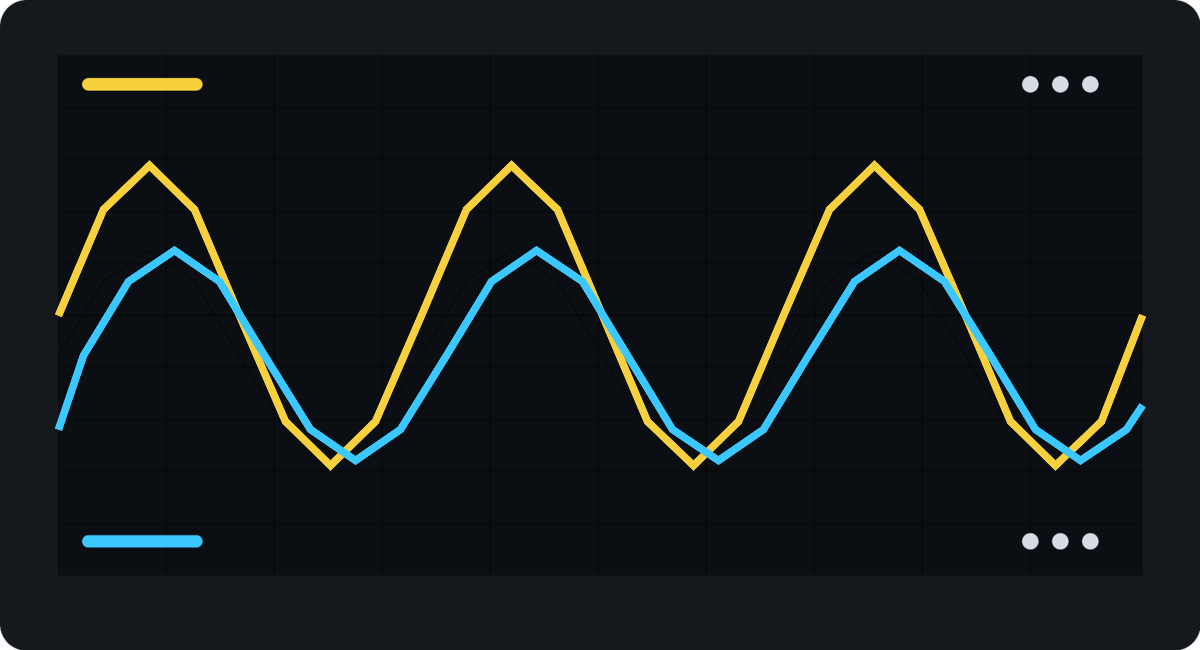
\includegraphics[width=0.82\linewidth]{oscilloscope-waveform.png}
  \caption{遮断周波数付近で観測した入力波形と出力波形}
  \label{fig:oscilloscope-waveform}
\end{figure}
% guide_image_end

\SampleGuideSource
  {外部画像を挿入するコード}
  {sections/03-method.tex}
  {guide_image_start}
  {guide_image_end}

\SampleGuideNote[orange!80!black]{［FIG-IMAGE-01］}{%
画像は \texttt{\string\includegraphics} で読み込みます。
ここでは \texttt{width=0.82\string\linewidth} とし、本文幅より少し小さく表示しています。}

\SampleGuideNote[orange!80!black]{画像パスの補足}{%
\texttt{report.tex} の \texttt{\string\graphicspath} により、ファイル名だけで \texttt{figures/} 内の画像を参照できます。}

% [DOC:LINK-HYPERREF-01] Hidden-border links for references and URLs.
\SampleGuideNote[orange!80!black]{ハイパーリンクの補足}{%
図番号や文献 URL には \texttt{hyperref} がリンクを付けますが、\texttt{hidelinks} により枠線は表示されません。}

\subsection{測定条件}
\label{subsec:conditions}

測定中に一定とする条件を以下に示す。

% [DOC:LIST-ITEMIZE-03] Measurement conditions.
\begin{itemize}[leftmargin=3em,itemsep=0.25em]
  \item 入力波形は正弦波とし、入力振幅は \qty{1.00}{\volt} に保つ。
  \item 周波数は低い側から高い側へ変化させ、遮断周波数付近では測定間隔を小さくする。
  \item 各周波数で振幅と時間差を三回読み取る。
  \item 周波数変更後は波形が安定してから記録する。
  \item 入力と出力のグラウンドは共通にする。
\end{itemize}

\SampleGuideNote[teal!70!black]{条件整理の補足}{%
同じ \texttt{itemize} 環境を、目的だけでなく測定中に固定する条件の整理にも使用できます。}

\subsection{測定手順}
\label{subsec:procedure}

% [DOC:LIST-ENUMERATE-01] Numbered measurement procedure.
測定手順は次のとおりとした。
% guide_enumerate_start
\begin{enumerate}[label=(\arabic*),leftmargin=3em,itemsep=0.25em]
  \item 抵抗値と静電容量を三回測定し、平均値を求める。
  \item \cref{fig:rc-circuit}の回路を構成し、配線を目視確認する。
  \item 信号発生器を正弦波、\qty{100}{\hertz}、\qty{1.00}{\volt} に設定する。
  \item CH1 と CH2 の零点、電圧軸および時間軸を調整する。
  \item \qty{100}{\hertz} から \qty{10}{\kilo\hertz} まで周波数を変化させ、振幅と時間差を記録する。
  \item \qtyrange{1.30}{2.00}{\kilo\hertz} では測定点を追加する。
  \item \qty{2.00}{\kilo\hertz} から \qty{500}{\hertz} まで逆方向にも測定し、走査方向の差を確認する。
  \item 測定終了後に入力を停止し、回路を取り外す。
\end{enumerate}
% guide_enumerate_end

\SampleGuideSource
  {番号付きの手順を書くコード}
  {sections/03-method.tex}
  {guide_enumerate_start}
  {guide_enumerate_end}

\SampleGuideNote[teal!70!black]{［LIST-ENUMERATE-01］}{%
順番が大切な手順には \texttt{enumerate} を使います。
\texttt{label=(\string\arabic*)} を付けると、番号を「(1)」の形にできます。}

\subsection{データの保存形式}
\label{subsec:data-format}

測定値は CSV ファイルへ保存した。各列の意味を以下に示す。

% [DOC:LIST-DESCRIPTION-03] Description list for CSV fields.
\begin{description}[leftmargin=12em,labelwidth=10.5em,nosep]
  \item[\texttt{frequency\_hz}] 入力周波数（\unit{\hertz}）
  \item[\texttt{gain\_measured}] 測定した利得（\unit{\decibel}）
  \item[\texttt{gain\_theory}] 素子値から計算した利得（\unit{\decibel}）
  \item[\texttt{phase\_measured}] 測定した位相差（\unit{\degree}）
  \item[\texttt{phase\_theory}] 理論式から計算した位相差（\unit{\degree}）
  \item[\texttt{residual\_db}] 測定利得と理論利得の差（\unit{\decibel}）
\end{description}

ファイル名は \lstinline|frequency-response.csv| とし、解析プログラムから同じ名前で読み込んだ。

% [DOC:CODE-INLINE-01] Inline code fragment.
\SampleGuideNote[red!65!black]{［CODE-INLINE-01］}{%
本文中の短いファイル名や変数名は、\texttt{listings} の \texttt{\string\lstinline} で等幅表示できます。}

% SAMPLE-ONLY: \SampleGuideNote and \SampleGuideSource are not template commands.
\section{実験結果}
\label{sec:results}

\subsection{周波数応答の測定値}
\label{subsec:response-data}

各周波数で得られた入力振幅、出力振幅、利得および位相差を
\cref{tab:frequency-response}に示す。入力振幅は全測定点で
$1.00\,\mathrm{V}$ に調整した。

% [DOC:TABLE-MULTIROW-01] Frequency bands grouped by multirow.
% guide_multirow_table_start
\begin{table}[htbp]
  \centering
  \caption{周波数応答の測定結果}
  \label{tab:frequency-response}
  \small
  \setlength{\tabcolsep}{3.5pt}
  \begin{tabularx}{\linewidth}{
      >{\centering\arraybackslash}p{0.12\linewidth}
      >{\centering\arraybackslash}p{0.13\linewidth}
      >{\centering\arraybackslash}p{0.11\linewidth}
      >{\centering\arraybackslash}p{0.11\linewidth}
      >{\centering\arraybackslash}p{0.13\linewidth}
      >{\centering\arraybackslash}X}
    \toprule
    領域 & 周波数 / Hz & 入力 / V & 出力 / V & 利得 / dB & 位相差 / deg \\
    \midrule
    \multirow{5}{*}{通過域}
      & 100  & 1.00 & 1.00 & $0.00$  & $-4$ \\
      & 200  & 1.00 & 0.99 & $-0.09$ & $-7$ \\
      & 300  & 1.00 & 0.98 & $-0.17$ & $-11$ \\
      & 500  & 1.00 & 0.96 & $-0.35$ & $-18$ \\
      & 700  & 1.00 & 0.92 & $-0.73$ & $-24$ \\
    \midrule
    \multirow{6}{*}{遷移域}
      & 1000 & 1.00 & 0.85 & $-1.41$ & $-33$ \\
      & 1300 & 1.00 & 0.78 & $-2.20$ & $-40$ \\
      & 1500 & 1.00 & 0.73 & $-2.78$ & $-44$ \\
      & 1600 & 1.00 & 0.70 & $-3.10$ & $-46$ \\
      & 1800 & 1.00 & 0.66 & $-3.61$ & $-49$ \\
      & 2000 & 1.00 & 0.62 & $-4.15$ & $-52$ \\
    \midrule
    \multirow{4}{*}{減衰域}
      & 3000  & 1.00 & 0.46 & $-6.70$  & $-62$ \\
      & 5000  & 1.00 & 0.30 & $-10.46$ & $-73$ \\
      & 7000  & 1.00 & 0.22 & $-13.05$ & $-77$ \\
      & 10000 & 1.00 & 0.16 & $-15.92$ & $-81$ \\
    \bottomrule
  \end{tabularx}
\end{table}
% guide_multirow_table_end

\SampleGuideSource
  {同じ分類を複数行にまとめる表のコード}
  {sections/04-results.tex}
  {guide_multirow_table_start}
  {guide_multirow_table_end}

\SampleGuideNote[orange!80!black]{［TABLE-MULTIROW-01］}{%
\texttt{multirow} を使うと、「通過域」のような同じ分類名を複数行にまとめて表示できます。
最初の数字には、まとめたい行数を指定します。}

\SampleGuideNote[orange!80!black]{表の幅に関する補足}{%
数値列には固定幅の \texttt{p} 列、最後の列には残り幅を使う \texttt{X} 列を組み合わせています。}

100--700 Hz では出力振幅が入力振幅に近く、利得の低下は
$1\,\mathrm{dB}$ 未満であった。1.30--2.00 kHz では利得と位相差が大きく変化し、
1.60 kHz で利得 $-3.10\,\mathrm{dB}$、位相差 $-46\,\mathrm{deg}$ を得た。
5 kHz 以上では出力振幅が明確に小さくなった。

\subsection{遮断周波数付近の繰り返し測定}
\label{subsec:repeatability}

遮断周波数付近の五つの周波数では、出力振幅を三回ずつ読み取った。
利得へ換算した結果と標準偏差を\cref{tab:repeatability}に示す。

% [DOC:TABLE-REPEAT-01] Ordinary table without multirow.
\begin{table}[H]
  \centering
  \caption{遮断周波数付近の繰り返し測定}
  \label{tab:repeatability}
  \begin{tabular}{rrrrrr}
    \toprule
    周波数 / Hz & 1 回目 / dB & 2 回目 / dB & 3 回目 / dB & 平均 / dB & 標準偏差 / dB \\
    \midrule
    1300 & $-2.18$ & $-2.22$ & $-2.20$ & $-2.20$ & 0.02 \\
    1500 & $-2.75$ & $-2.80$ & $-2.79$ & $-2.78$ & 0.03 \\
    1600 & $-3.08$ & $-3.12$ & $-3.10$ & $-3.10$ & 0.02 \\
    1800 & $-3.58$ & $-3.63$ & $-3.62$ & $-3.61$ & 0.03 \\
    2000 & $-4.12$ & $-4.18$ & $-4.15$ & $-4.15$ & 0.03 \\
    \bottomrule
  \end{tabular}
\end{table}

\SampleGuideNote[orange!80!black]{［TABLE-REPEAT-01］}{%
単純な数値の比較では標準の \texttt{tabular} も使用できます。ここでは列を右寄せして桁を比較しやすくしています。}

三回の測定値の標準偏差は $0.02$--$0.03\,\mathrm{dB}$ であり、
同じ条件での短時間の繰り返しに対しては大きなばらつきは見られなかった。

\subsection{単一縦軸の利得特性}
\label{subsec:single-axis-plot}

まず、利得だけを単一の縦軸で比較した結果を\cref{fig:gain-response}に示す。
測定値と理論値には同じ CSV ファイルの別々の列を用いた。

% [DOC:PLOT-SINGLE-01] Single-axis PGFPlots figure.
% [DOC:PLOT-DATAFILE-01] Data read from a CSV file.
% [DOC:PLOT-STYLE-LEGEND-01] Legend styling included by report axis.
% Fixed placement keeps each plot next to its annotation.
% guide_single_plot_start
\begin{figure}[H]
  \centering
  \begin{tikzpicture}
    \begin{axis}[
      report axis,
      width=0.82\linewidth,
      height=0.52\linewidth,
      xmode=log,
      xmin=80,
      xmax=12000,
      ymin=-18,
      ymax=1,
      xtick={100,1000,10000},
      xticklabels={$10^2$,$10^3$,$10^4$},
      ytick={-15,-10,-5,0},
      xlabel={周波数 / Hz},
      ylabel={利得 / dB}
    ]
      \addplot[report plot,mark=*]
        table[x=frequency_hz,y=gain_measured,col sep=comma]
        {data/frequency-response.csv};
      \addlegendentry{測定値}
      \addplot[report plot,dashed,mark=none]
        table[x=frequency_hz,y=gain_theory,col sep=comma]
        {data/frequency-response.csv};
      \addlegendentry{理論値}
    \end{axis}
  \end{tikzpicture}
  \caption{利得の周波数特性}
  \label{fig:gain-response}
\end{figure}
% guide_single_plot_end

\SampleGuideSource
  {CSV から一つのグラフを作るコード}
  {sections/04-results.tex}
  {guide_single_plot_start}
  {guide_single_plot_end}

% [DOC:PLOT-STYLE-AXIS-01] Shared axis and legend style.
% [DOC:PLOT-STYLE-PLOT-01] Shared series style.
\SampleGuideNote[orange!80!black]{［PLOT-SINGLE-01］}{%
一つの \texttt{axis} の中に二つの \texttt{\string\addplot} を書き、
測定値と理論値を同じグラフで比べています。}

\SampleGuideNote[orange!80!black]{［PLOT-STYLE-AXIS-01］}{%
\texttt{report axis} は軸線、目盛、グリッド、ラベル、凡例を共通書式にそろえます。}

\SampleGuideNote[orange!80!black]{［PLOT-STYLE-PLOT-01］}{%
測定系列に \texttt{report plot} を指定すると、線幅とマーカーの大きさを統一できます。}

\SampleGuideNote[orange!80!black]{データ読み込みの補足}{%
\texttt{\string\addplot table} は CSV の列名を指定して、外部データファイルから座標を読み込みます。}

\SampleGuideNote[orange!80!black]{凡例スタイルの補足}{%
\texttt{report legend} は、凡例の位置、枠線、文字サイズをまとめてそろえます。}

% [DOC:PLOT-LOG-01] Logarithmic frequency axis.
\SampleGuideNote[orange!80!black]{対数軸の補足}{%
周波数軸には \texttt{xmode=log} を指定し、100 Hz、1 kHz、10 kHz を等間隔に表示しています。}

測定値は全周波数範囲で理論曲線に沿って変化した。
特に遮断周波数付近では、測定点を増やしたことにより曲線の変化を細かく確認できた。

\subsection{利得と位相差の二重縦軸表示}
\label{subsec:dual-axis-plot}

利得と位相差を同じ周波数軸で比較した結果を\cref{fig:dual-response}に示す。

% [DOC:PLOT-DUAL-01] Two overlaid axes with a right-hand y-axis.
\begin{figure}[H]
  \centering
  \begin{tikzpicture}
    \begin{axis}[
      report axis,
      name=gainaxis,
      width=0.78\linewidth,
      height=0.48\linewidth,
      xmode=log,
      xmin=80,
      xmax=12000,
      ymin=-18,
      ymax=1,
      xtick={100,1000,10000},
      xticklabels={$10^2$,$10^3$,$10^4$},
      ytick={-15,-10,-5,0},
      xlabel={周波数 / Hz},
      ylabel={利得 / dB},
      legend style={at={(0.03,0.04)},anchor=south west}
    ]
      \addplot[report plot,mark=*]
        table[x=frequency_hz,y=gain_measured,col sep=comma]
        {data/frequency-response.csv};
      \addlegendentry{利得（測定）}
      \addplot[report plot,dashed,mark=none]
        table[x=frequency_hz,y=gain_theory,col sep=comma]
        {data/frequency-response.csv};
      \addlegendentry{利得（理論）}
      \addplot[black!55,densely dotted,line width=0.8pt,mark=none]
        coordinates {(1580,-18) (1580,1)};
    \end{axis}
    % guide_dual_right_axis_start
    \begin{axis}[
      report dual right axis,
      width=0.78\linewidth,
      height=0.48\linewidth,
      xmode=log,
      xmin=80,
      xmax=12000,
      ymin=-90,
      ymax=0,
      ytick={-90,-60,-30,0},
      ylabel={位相差 / deg},
      legend style={at={(0.97,0.96)},anchor=north east}
    ]
      \addplot[blue!60!black,line width=1.2pt,mark=square*,mark size=2.1pt]
        table[x=frequency_hz,y=phase_measured,col sep=comma]
        {data/frequency-response.csv};
      \addlegendentry{位相差（測定）}
      \addplot[blue!60!black,dashed,line width=1.0pt,mark=none]
        table[x=frequency_hz,y=phase_theory,col sep=comma]
        {data/frequency-response.csv};
      \addlegendentry{位相差（理論）}
    \end{axis}
    % guide_dual_right_axis_end
  \end{tikzpicture}
  \caption{利得と位相差の周波数特性}
  \label{fig:dual-response}
\end{figure}

\SampleGuideSource
  {右側の縦軸を重ねるコード}
  {sections/04-results.tex}
  {guide_dual_right_axis_start}
  {guide_dual_right_axis_end}

% [DOC:PLOT-STYLE-RIGHT-01] Right-hand axis style.
\SampleGuideNote[orange!80!black]{［PLOT-DUAL-01］}{%
同じ \texttt{tikzpicture} に二つの \texttt{axis} を重ねると、
左側と右側に別の縦軸を持つグラフを作れます。}

\SampleGuideNote[orange!80!black]{［PLOT-STYLE-RIGHT-01］}{%
右側の軸に \texttt{report dual right axis} を指定すると、左側のグラフに重ねやすい書式になります。}

\SampleGuideNote[orange!80!black]{軸を重ねるときの補足}{%
二つの軸で幅、高さ、横軸範囲を同じ値にすると、目盛位置が正確に一致します。}

\Crefrange{fig:gain-response}{fig:dual-response}から、利得と位相差のどちらを用いても
遮断周波数が 1.6 kHz 付近にあることを確認できる。

\subsection{利得残差}
\label{subsec:residuals}

測定利得から理論利得を引いた残差を\cref{fig:gain-residual}に示す。

% [DOC:PLOT-BASE-01] Base axis style without a legend.
\begin{figure}[H]
  \centering
  \begin{tikzpicture}
    \begin{axis}[
      report axis base,
      width=0.78\linewidth,
      height=0.42\linewidth,
      xmode=log,
      xmin=80,
      xmax=12000,
      ymin=-0.20,
      ymax=0.20,
      xtick={100,1000,10000},
      xticklabels={$10^2$,$10^3$,$10^4$},
      ytick={-0.2,-0.1,0,0.1,0.2},
      xlabel={周波数 / Hz},
      ylabel={利得残差 / dB}
    ]
      \addplot[report plot,only marks,mark=*]
        table[x=frequency_hz,y=residual_db,col sep=comma]
        {data/frequency-response.csv};
      \addplot[black,dashed,line width=0.7pt,mark=none]
        coordinates {(80,0) (12000,0)};
    \end{axis}
  \end{tikzpicture}
  \caption{測定利得と理論利得の残差}
  \label{fig:gain-residual}
\end{figure}

\SampleGuideNote[orange!80!black]{［PLOT-BASE-01］}{%
凡例を必要としないグラフでは、軸の基本書式だけを持つ \texttt{report axis base} を直接利用できます。}

残差は $-0.10$--$0.15\,\mathrm{dB}$ の範囲にあり、特定の周波数だけが
大きく外れる傾向は見られなかった。
\cref{tab:frequency-response,tab:repeatability,fig:gain-residual}を合わせると、
測定値のばらつきよりも周波数ごとのわずかな系統差が残っていることが分かる。

% [DOC:REF-MULTI-01] Mixed-type multi-label reference.
\SampleGuideNote[blue!65!black]{［REF-MULTI-01］}{%
種類の異なる複数ラベルを一つの \texttt{\string\cref} に指定すると、表と図の名称を自動で分けて表示します。}

% SAMPLE-ONLY: \SampleGuideNote and \SampleGuideSource are not template commands.
\section{考察}
\label{sec:discussion}

\subsection{データ処理}
\label{subsec:data-processing}

CSV ファイルから周波数、利得、位相差を読み込み、理論値との差を計算した。
\Cref{lst:analysis}に、読み込みと基本計算の処理を示す。

% [DOC:CODE-BLOCK-01] Python listing with comments, strings, numbers, and wrapping.
% guide_listing_start
\begin{lstlisting}[
  language=Python,
  caption={周波数応答データの読み込みと基本計算},
  label={lst:analysis}
]
import csv
import math

INPUT_FILE = "data/frequency-response.csv"

with open(INPUT_FILE, encoding="utf-8") as stream:
    rows = list(csv.DictReader(stream))

# Convert selected CSV fields from text to floating-point values.
measurements = [
    {
        "frequency": float(row["frequency_hz"]),
        "gain": float(row["gain_measured"]),
        "phase": float(row["phase_measured"]),
    }
    for row in rows
]

gain_cutoff = min(
    measurements,
    key=lambda row: abs(row["gain"] + 3.0),
)

message = (
    f"nearest cutoff candidate: {gain_cutoff['frequency']:.0f} Hz, "
    f"gain={gain_cutoff['gain']:.2f} dB, phase={gain_cutoff['phase']:.1f} deg"
)
print(message)
\end{lstlisting}
% guide_listing_end

\SampleGuideSource
  {コードを本文に載せるための LaTeX ソース}
  {sections/05-discussion.tex}
  {guide_listing_start}
  {guide_listing_end}

\SampleGuideNote[red!65!black]{［CODE-BLOCK-01］}{%
\texttt{lstlisting} の中にプログラムを書くと、コード用の書体と枠で表示できます。
\texttt{caption} には見出し、\texttt{label} には参照用の名前を書きます。}

% [DOC:CODE-HIGHLIGHT-01] Syntax highlighting by language.
\SampleGuideNote[red!65!black]{［CODE-HIGHLIGHT-01］}{%
\texttt{language=Python} により、予約語、コメント、文字列が種類ごとに色分けされます。}

% [DOC:CODE-WRAP-01] Automatic wrapping of long source lines.
\SampleGuideNote[red!65!black]{長い行の補足}{%
枠幅を超えるコードは、全体設定の \texttt{breaklines=true} により次の行へ折り返されます。}

% [DOC:CODE-REF-01] Cross-reference to a listing label.
\SampleGuideNote[red!65!black]{コード参照の補足}{%
\texttt{caption} と \texttt{label} を付けたコードは、図や表と同様に \texttt{\string\cref} から参照できます。}

\subsection{利得から求めた遮断周波数}
\label{subsec:gain-cutoff}

$-3\,\mathrm{dB}$ をはさむ 1.50 kHz と 1.60 kHz の二点を用い、
利得を周波数に対して線形補間した。補間処理を\cref{lst:interpolation}に示す。

% [DOC:CODE-BLOCK-02] A second Python listing.
\begin{lstlisting}[
  language=Python,
  caption={二点間の線形補間},
  label={lst:interpolation}
]
def interpolate_x(x1, y1, x2, y2, target_y):
    ratio = (target_y - y1) / (y2 - y1)
    return x1 + ratio * (x2 - x1)

cutoff_gain_hz = interpolate_x(
    1500.0, -2.78,
    1600.0, -3.10,
    -3.00,
)

print(f"gain estimate = {cutoff_gain_hz:.1f} Hz")
\end{lstlisting}

得られた遮断周波数は $1.57\,\mathrm{kHz}$ であった。
測定点を一つ選ぶだけの場合は 1.60 kHz となるが、二点補間により理論値へ近い値が得られた。

\subsection{位相差から求めた遮断周波数}
\label{subsec:phase-cutoff}

位相差が $-45\,\mathrm{deg}$ となる点についても、1.50 kHz の
$-44\,\mathrm{deg}$ と 1.60 kHz の $-46\,\mathrm{deg}$ の間を補間した。
この方法による遮断周波数は $1.55\,\mathrm{kHz}$ となった。

利得による推定値と位相差による推定値の差は 20 Hz であった。
この差は、振幅と時間差を別々に読み取ったこと、および表示分解能が異なることにより生じたと考えられる。

\subsection{曲線全体を用いた推定}
\label{subsec:curve-fit}

全測定点に対して理論式の $f_c$ だけを変化させ、利得残差の二乗和が最小となる値を探索した。
実行時に用いたコマンドを\cref{lst:run-command}に示す。

% [DOC:CODE-LANGUAGE-02] Bash listing.
\begin{lstlisting}[
  language=bash,
  caption={解析プログラムの実行コマンド},
  label={lst:run-command}
]
python3 analyze_response.py \
  --input data/frequency-response.csv \
  --fit gain \
  --output build/fit-summary.txt
\end{lstlisting}

\SampleGuideNote[red!65!black]{［CODE-LANGUAGE-02］}{%
\texttt{language} の値を変更すると、同じ \texttt{lstlisting} で別の言語の構文を表示できます。}

曲線全体から得られた遮断周波数は $1.58\,\mathrm{kHz}$ であった。
三つの推定結果を\cref{tab:cutoff-estimates}にまとめる。

\begin{table}[H]
  \centering
  \caption{遮断周波数の推定結果}
  \label{tab:cutoff-estimates}
  \begin{tabularx}{0.88\linewidth}{
      >{\raggedright\arraybackslash}p{0.26\linewidth}
      >{\centering\arraybackslash}p{0.18\linewidth}
      >{\raggedright\arraybackslash}X}
    \toprule
    推定方法 & 推定値 / kHz & 使用した情報 \\
    \midrule
    利得の二点補間 & 1.57 & $-3\,\mathrm{dB}$ をはさむ 1.50 kHz と 1.60 kHz の測定値 \\
    位相差の二点補間 & 1.55 & $-45\,\mathrm{deg}$ をはさむ二つの位相差 \\
    利得曲線の当てはめ & 1.58 & 100 Hz から 10 kHz までの全利得測定値 \\
    \bottomrule
  \end{tabularx}
\end{table}

三つの値は 1.55--1.58 kHz の範囲にあり、素子の測定値から求めた
理論値 $1.58\,\mathrm{kHz}$ と近かった。

\subsection{理論値との差}
\label{subsec:relative-error}

代表値として曲線当てはめによる $1.58\,\mathrm{kHz}$ を用い、
公称値から求めた $1.59\,\mathrm{kHz}$ との相対差を\cref{eq:relative-error}で計算した。

\begin{equation}
  \varepsilon
  =\frac{\lvert 1.58-1.59\rvert}{1.59}\times100
  \simeq0.63\,\%
  \label{eq:relative-error}
\end{equation}

一方、実測した $R=0.998\,\mathrm{k}\Omega$、$C=0.101\,\mu\mathrm{F}$ を
\cref{eq:cutoff}に代入した値は $1.58\,\mathrm{kHz}$ であり、曲線当てはめの値と一致した。

\subsection{素子公差の影響}
\label{subsec:tolerance-discussion}

\crefrange{eq:cutoff-min}{eq:cutoff-max}で求めた 1.49--1.71 kHz の範囲には、
三つの推定値がすべて含まれる。一次近似では、遮断周波数の相対変化は
抵抗と静電容量の相対変化の和に対応する。

\begin{align}
  \frac{\Delta f_c}{f_c}
    &\simeq-\frac{\Delta R}{R}-\frac{\Delta C}{C}
      \label{eq:tolerance-propagation}\\
  \left\lvert\frac{\Delta f_c}{f_c}\right\rvert
    &\leq
      \left\lvert\frac{\Delta R}{R}\right\rvert
      +\left\lvert\frac{\Delta C}{C}\right\rvert.
      \label{eq:tolerance-bound}
\end{align}

測定した抵抗値のずれは小さく、今回の遮断周波数には主に静電容量のずれが影響したと考えられる。
素子公差を含む測定不確かさの整理には、学位論文で示された方法も参照した\cite{jp-thesis}。

\subsection{測定器による負荷}
\label{subsec:instrument-loading}

理論式では信号発生器を理想電圧源、オシロスコープを無限大の入力抵抗として扱った。
実際には信号発生器に $50\,\Omega$ の出力抵抗があり、プローブにも入力抵抗と入力容量がある。
そのため、回路から見た実効抵抗と実効容量は公称値だけで決まらない。

特に高周波側ではプローブの入力容量がコンデンサと並列に加わり、
理論曲線よりわずかに大きな減衰を生じる可能性がある。
\cref{fig:gain-residual}で 10 kHz の残差が正側へずれたことには、
振幅読取りの分解能や信号発生器の出力変化も影響したと考えられる。

\subsection{走査方向と再現性}
\label{subsec:sweep-direction}

500 Hz から 2.00 kHz までを逆方向にも測定した結果、同じ周波数での利得差は
最大 $0.04\,\mathrm{dB}$ であった。RC 回路は受動回路であり、今回の時間間隔では
明確な履歴依存性は見られなかった。

ただし、周波数を切り替えた直後に値を読み取ると、オシロスコープの自動測定値が
一時的に変動することがあった。測定許可信号の考え方や同期測定については、
講演資料と会議録の整理も参照した\cite{jp-inproceedings,jp-proceedings}。

\subsection{主な誤差要因}
\label{subsec:error-sources}

理論値と測定値の差に含まれる要因を以下にまとめる。

% [DOC:LIST-DESCRIPTION-04] Description list for error sources.
\begin{description}[leftmargin=10em,labelwidth=8.5em,itemsep=0.25em]
  \item[素子の公差] 抵抗値と静電容量が公称値からずれる。
  \item[周波数間隔] 真の $-3\,\mathrm{dB}$ 点を直接測定せず、測定点間を補間している。
  \item[出力抵抗] 信号発生器の $50\,\Omega$ を単純な理論式に含めていない。
  \item[プローブ負荷] プローブの入力抵抗と入力容量が回路へ加わる。
  \item[時間差読取り] カーソル位置の分解能が位相差へ変換される。
  \item[振幅読取り] 高周波側では出力振幅が小さく、相対的な読取り誤差が増える。
\end{description}

実験室内の事前メモに記録された注意点とも比較し、グラウンド接続とプローブ倍率を
毎回確認する必要があると判断した\cite{jp-unpublished}。
英語文献に示された一次フィルタの評価方法とも、測定手順と結果の傾向は一致した\cite{en-article}。

\subsection{測定方法の改善案}
\label{subsec:improvements}

次回の測定では、以下の順に条件を改善する。

% [DOC:LIST-ENUMERATE-02] A second enumerate example.
\begin{enumerate}[label=\arabic*.,leftmargin=3em,itemsep=0.35em]
  \item 1.45--1.70 kHz の測定間隔を 25 Hz 程度まで小さくする。
  \item 各周波数で五回以上測定し、平均値と標準不確かさを求める。
  \item 信号発生器の出力抵抗を含む等価回路で理論値を計算する。
  \item プローブの入力容量を実測または仕様値から補正する。
  \item 自動保存した波形から振幅と位相差を同じ処理で計算する。
\end{enumerate}

\SampleGuideNote[teal!70!black]{番号形式の補足}{%
二つ目の \texttt{enumerate} では \texttt{label=\string\arabic*.} とし、通常の「1.」形式を使用しています。}

% SAMPLE-ONLY: \SampleGuideNote adds PDF guidance and is not a template command.
\section{まとめ}
\label{sec:summary}

本実験では、抵抗とコンデンサから構成される一次 RC 低域通過フィルタを作製し、
100 Hz から 10 kHz までの周波数応答を測定した。
入力振幅を $1.00\,\mathrm{V}$ に保ち、出力振幅と入出力波形の時間差から
利得と位相差を求めた。

低周波数側では利得が $0\,\mathrm{dB}$ に近く、入力信号がほぼ保たれた。
周波数の増加に伴って利得は低下し、位相差は $-90\,\mathrm{deg}$ に近づいた。
この変化は\cref{fig:gain-response,fig:dual-response}に示した理論曲線と同じ傾向であった。

遮断周波数は、利得の二点補間から 1.57 kHz、位相差の二点補間から 1.55 kHz、
利得曲線全体の当てはめから 1.58 kHz と推定された。
測定した素子値から計算した値は 1.58 kHz であり、曲線全体を用いた推定値と一致した。

主な定量結果を以下にまとめる。

% [DOC:LIST-ITEMIZE-04] Quantitative summary list.
\begin{itemize}[leftmargin=3em,itemsep=0.3em]
  \item $1.60\,\mathrm{kHz}$ における利得：$-3.10\,\mathrm{dB}$
  \item $1.60\,\mathrm{kHz}$ における位相差：$-46\,\mathrm{deg}$
  \item 曲線当てはめによる遮断周波数：$1.58\,\mathrm{kHz}$
  \item 公称素子値から求めた値との相対差：$0.63\,\%$
  \item 遮断周波数付近の利得標準偏差：$0.02$--$0.03\,\mathrm{dB}$
\end{itemize}

\SampleGuideNote[teal!70!black]{まとめの一覧に関する補足}{%
定量結果だけを短く再掲する場合にも、\texttt{itemize} を使用して本文と数値を分けられます。}

理論値と測定値の小さな差には、素子値の公差、測定周波数の間隔、
信号発生器の出力抵抗、プローブの入力容量、振幅と時間差の読取り分解能が含まれる。
三回の繰り返し測定では大きなばらつきは見られなかったが、系統的な差をさらに評価するには、
測定点を増やし、測定器の等価回路を理論計算へ取り入れる必要がある。

以上より、一次 RC 低域通過フィルタの振幅特性と位相特性を同じ測定から確認し、
素子値、表形式の測定結果、グラフおよび解析コードを対応させて遮断周波数を評価できた。

% SAMPLE-ONLY: \SampleGuideNote and \SampleGuideSource are not template commands.
% [DOC:BIB-CONDITION-01] Print the bibliography only when data was cited.
\iflabreporthasreferences
  \SampleGuideSource
    {オンライン資料を登録する BibLaTeX データ}
    {bibliography/references.bib}
    {guide_bib_entry_start}
    {guide_bib_entry_end}

  % [DOC:BIB-JAPANESE-01] Japanese bibliography selection with langid.
  \par\smallskip
  \SampleGuideNote[violet!70!black]{［BIB-JAPANESE-01］}{%
日本語文献に \texttt{langid=\{japanese\}} を指定すると、
    \texttt{biblatex-jareport} の日本語書式が選択されます。}

  % [DOC:BIB-DRIVERS-01] Overview of the Japanese entry-type drivers.
  \SampleGuideNote[violet!70!black]{［BIB-DRIVERS-01］}{%
以下の一覧には、書籍、論文、分担章、会議論文、会議録、報告書、学位論文、
    オンライン資料、技術資料、未刊行資料の各形式を含めています。}

  % English entries use the fallback style.
  \SampleGuideNote[violet!70!black]{英語文献の補足}{%
英語文献では日本語用の書式を使わず、この例では IEEE 形式で出力されます。}

  % [DOC:BIB-URL-01] URL and access date fields.
  \SampleGuideNote[violet!70!black]{URL の補足}{%
\texttt{online} などの文献では、\texttt{url} と \texttt{urldate} から URL と参照日を出力できます。}

  % [DOC:BIB-COMPRESS-01] Numeric citation compression.
  \SampleGuideNote[violet!70!black]{引用番号の補足}{%
\texttt{citestyle=numeric-comp} により、連続する複数文献の引用番号は範囲へ圧縮されます。}

  \SampleGuideNote[violet!70!black]{［BIB-CONDITION-01］}{%
このテンプレートでは、本文で引用した文献がある場合だけ参考文献一覧を表示します。}
  \smallskip

  % [DOC:BIB-PRINT-01]
  \printbibliography[title={参考文献}]
\fi


\end{document}
